\documentclass[tikz,border=0pt]{standalone}
\usetikzlibrary{calc}
% Palette: the 3D gym's colours (crates/core/src/mesh.rs, data/shaders/scene.frag).
\definecolor{sky}{HTML}{DCE6EE}
\definecolor{skyhi}{HTML}{F2F6F9}
\definecolor{wall}{HTML}{EDE6D3}
\definecolor{walldark}{HTML}{D6CCB4}
\definecolor{stripeblue}{HTML}{2F5CBF}
\definecolor{stripegold}{HTML}{F8C537}
\definecolor{window}{HTML}{CFE6FF}
\definecolor{windowlit}{HTML}{F6FBFF}
\definecolor{wood}{HTML}{DBA86B}
\definecolor{wooddark}{HTML}{B98549}
\definecolor{woodline}{HTML}{C9965A}
\definecolor{mat}{HTML}{2961CC}
\definecolor{matlit}{HTML}{4A82E8}
\definecolor{matdark}{HTML}{1C4597}
\definecolor{matseam}{HTML}{16377A}
\definecolor{red}{HTML}{DD3D38}
\definecolor{redlit}{HTML}{F06A5E}
\definecolor{reddark}{HTML}{A92A27}
\definecolor{yellow}{HTML}{F9C02E}
\definecolor{yellowlit}{HTML}{FFDB6B}
\definecolor{yellowdark}{HTML}{C9961C}
\definecolor{green}{HTML}{3FA866}
\definecolor{greenlit}{HTML}{62C98A}
\definecolor{greendark}{HTML}{2C7D4B}
\definecolor{pink}{HTML}{F27A93}
\definecolor{pinklit}{HTML}{F7A1B3}
\definecolor{orange}{HTML}{F28A2E}
\definecolor{orangelit}{HTML}{F7AE66}
\definecolor{orangedark}{HTML}{C2671A}
\definecolor{sky2}{HTML}{7FB8F0}
\definecolor{purple}{HTML}{8B5CC8}
\definecolor{skin}{HTML}{F2C49A}
\definecolor{skinlit}{HTML}{F8D8B8}
\definecolor{skindark}{HTML}{D9A47A}
\definecolor{skinb}{HTML}{B9835A}
\definecolor{skinbdark}{HTML}{93653F}
\definecolor{shirt}{HTML}{E2463F}
\definecolor{shirtdark}{HTML}{B23430}
\definecolor{shirtb}{HTML}{2F7DD8}
\definecolor{shirtbdark}{HTML}{225DA6}
\definecolor{shorts}{HTML}{21305A}
\definecolor{shortsdark}{HTML}{151F3D}
\definecolor{shoe}{HTML}{FFFFFF}
\definecolor{shoedark}{HTML}{D8DDE3}
\definecolor{hair}{HTML}{4A2F1C}
\definecolor{band}{HTML}{F8C537}
\definecolor{chick}{HTML}{FBE48F}
\definecolor{chicklit}{HTML}{FFF2BE}
\definecolor{chickdark}{HTML}{DCC064}
\definecolor{comb}{HTML}{E2302E}
\definecolor{beak}{HTML}{F28A2E}
\definecolor{noodle}{HTML}{57D163}
\definecolor{noodledark}{HTML}{3A9E45}
\definecolor{ball}{HTML}{D8302B}
\definecolor{balldark}{HTML}{A5211D}
\definecolor{balllit}{HTML}{F0645D}
\definecolor{duck}{HTML}{FFD12E}
\definecolor{duckdark}{HTML}{E0A814}
\definecolor{foam}{HTML}{2F6BE0}
\definecolor{foamdark}{HTML}{214FAD}
\definecolor{white}{HTML}{FFFFFF}
\definecolor{ink}{HTML}{1E2B45}
\definecolor{netline}{HTML}{9AA9BF}
\definecolor{glow}{HTML}{FFF4C2}
\begin{document}
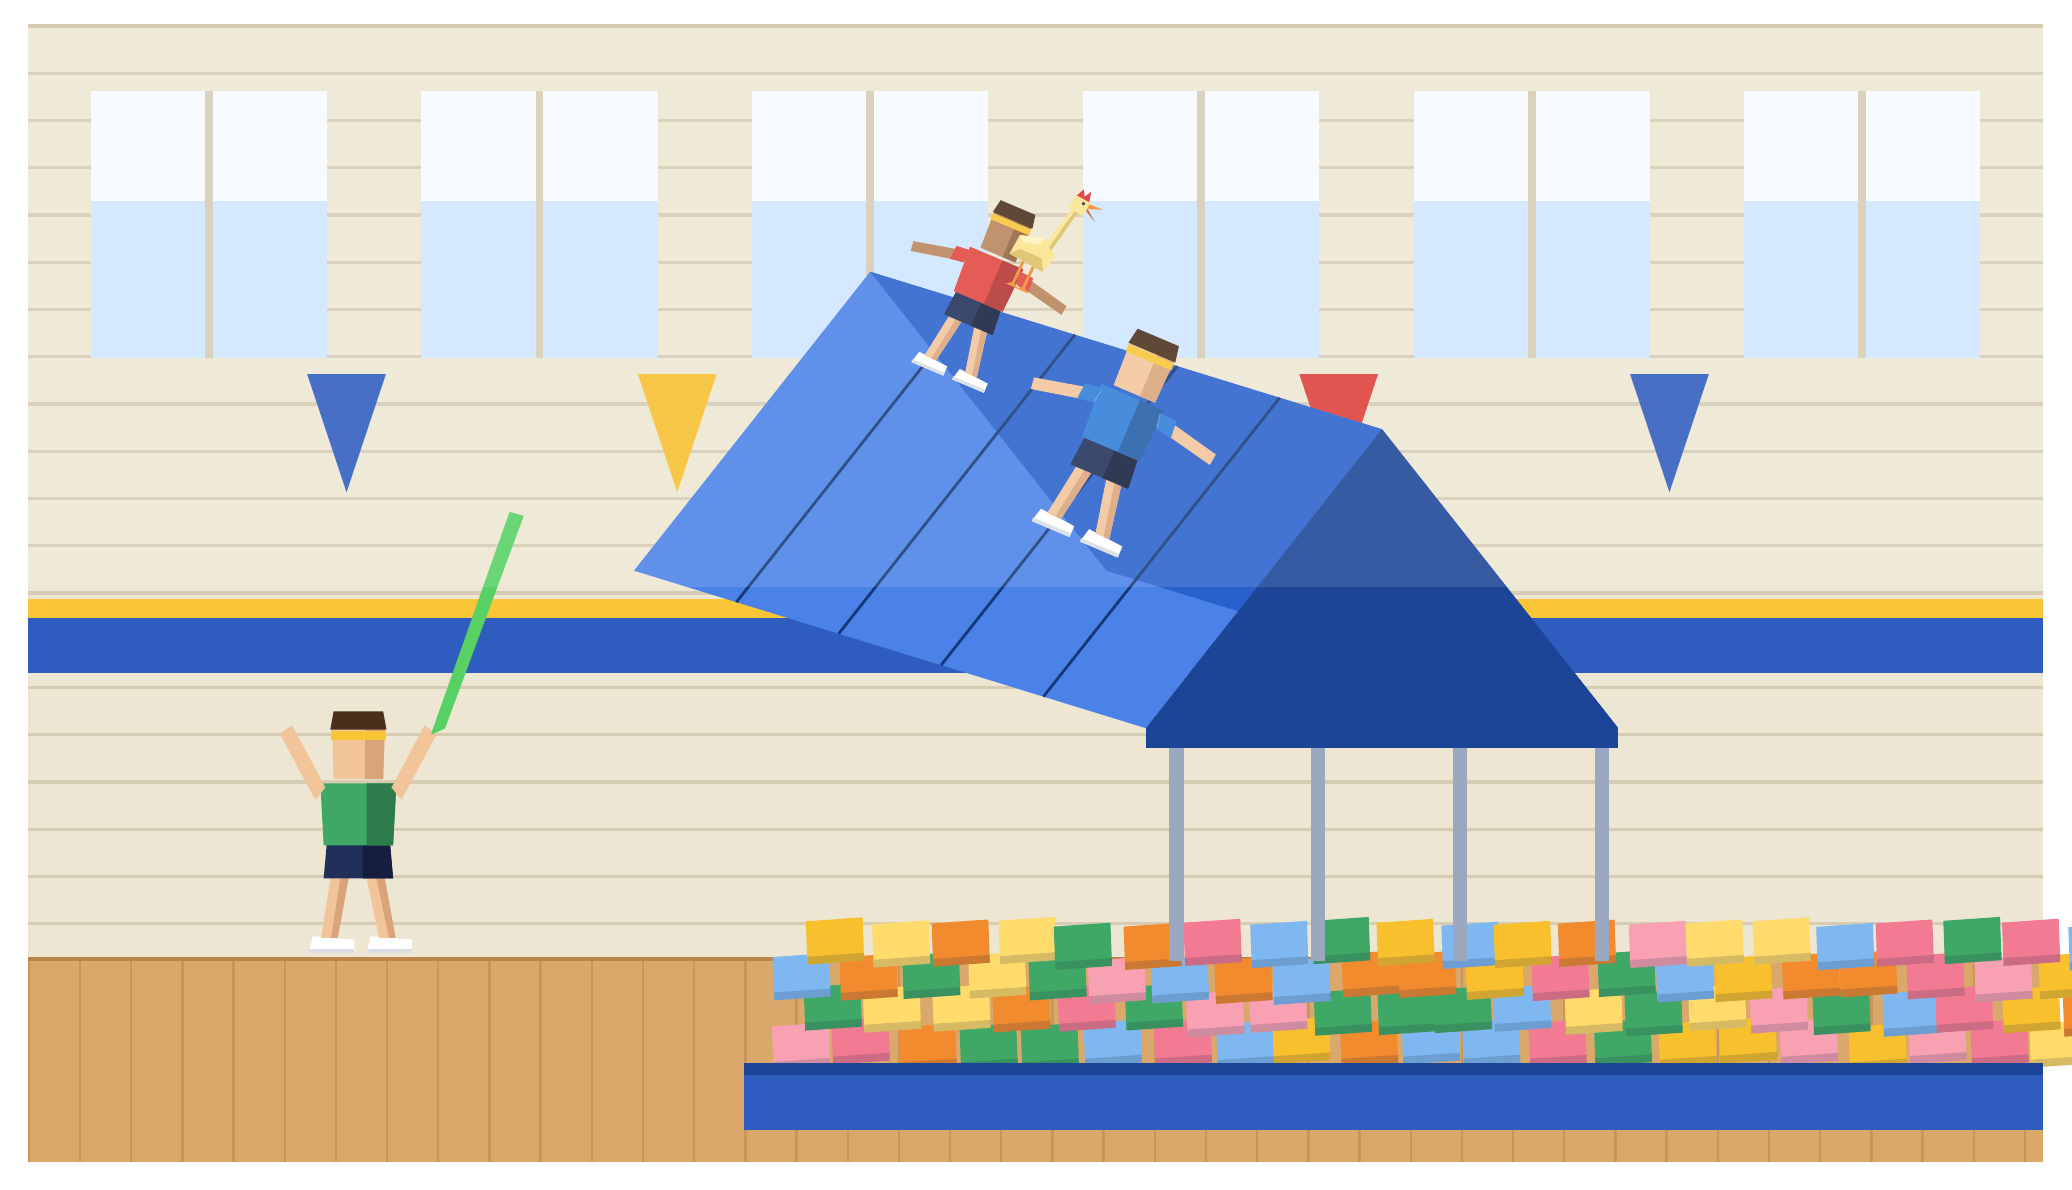
\begin{tikzpicture}[x=1cm,y=1cm]
\useasboundingbox (0,0) rectangle (25.6,14.4);
% ---- background: the gym wall, its stripe and high windows ----
\fill[wall] (0,0) rectangle (25.6,14.4);
\foreach \row in {0,...,24} {\fill[walldark] (0,{\row*0.6}) rectangle (25.6,{\row*0.6+0.04});}
\fill[stripeblue] (0,6.2) rectangle (25.6,6.9);
\fill[stripegold] (0,6.9) rectangle (25.6,7.15);
\foreach \i in {0,...,5} {\fill[window] ({0.8+\i*4.2},10.2) rectangle ({3.8+\i*4.2},13.6);\fill[windowlit] ({0.8+\i*4.2},12.2) rectangle ({3.8+\i*4.2},13.6);\fill[walldark] ({2.25+\i*4.2},10.2) rectangle ({2.35+\i*4.2},13.6);}
% pennants between the windows
\fill[stripeblue] (3.55,10) -- (4.55,10) -- (4.05,8.5) -- cycle;
\fill[yellow] (7.75,10) -- (8.75,10) -- (8.25,8.5) -- cycle;
\fill[green] (11.95,10) -- (12.95,10) -- (12.45,8.5) -- cycle;
\fill[red] (16.15,10) -- (17.15,10) -- (16.65,8.5) -- cycle;
\fill[stripeblue] (20.35,10) -- (21.35,10) -- (20.85,8.5) -- cycle;
% ---- the floor: maple boards ----
\fill[wood] (0,0) rectangle (25.6,2.6);
\foreach \i in {0,...,40} {\fill[woodline] ({\i*0.65},0) rectangle ({\i*0.65+0.03},2.6);}
\fill[wooddark] (0,2.55) rectangle (25.6,2.6);
% ---- the foam pit: a low wall and rows of foam cubes ----
\fill[pinklit] (9.472,1.165) -- (10.192,1.215) -- (10.172,1.765) -- (9.452,1.715) -- cycle;
\fill[ink,opacity=0.18] (9.472,1.165) -- (10.192,1.215) -- (10.192,1.315) -- (9.472,1.265) -- cycle;
\fill[pink] (10.228,1.232) -- (10.948,1.282) -- (10.928,1.832) -- (10.208,1.782) -- cycle;
\fill[ink,opacity=0.18] (10.228,1.232) -- (10.948,1.282) -- (10.948,1.382) -- (10.228,1.332) -- cycle;
\fill[orange] (11.079,1.156) -- (11.799,1.206) -- (11.779,1.756) -- (11.059,1.706) -- cycle;
\fill[ink,opacity=0.18] (11.079,1.156) -- (11.799,1.206) -- (11.799,1.306) -- (11.079,1.256) -- cycle;
\fill[green] (11.854,1.159) -- (12.574,1.209) -- (12.554,1.759) -- (11.834,1.709) -- cycle;
\fill[ink,opacity=0.18] (11.854,1.159) -- (12.574,1.209) -- (12.574,1.309) -- (11.854,1.259) -- cycle;
\fill[green] (12.631,1.159) -- (13.351,1.209) -- (13.331,1.759) -- (12.611,1.709) -- cycle;
\fill[ink,opacity=0.18] (12.631,1.159) -- (13.351,1.209) -- (13.351,1.309) -- (12.631,1.259) -- cycle;
\fill[sky2] (13.429,1.207) -- (14.149,1.257) -- (14.129,1.807) -- (13.409,1.757) -- cycle;
\fill[ink,opacity=0.18] (13.429,1.207) -- (14.149,1.257) -- (14.149,1.357) -- (13.429,1.307) -- cycle;
\fill[pink] (14.321,1.208) -- (15.041,1.258) -- (15.021,1.808) -- (14.301,1.758) -- cycle;
\fill[ink,opacity=0.18] (14.321,1.208) -- (15.041,1.258) -- (15.041,1.358) -- (14.321,1.308) -- cycle;
\fill[sky2] (15.112,1.19) -- (15.832,1.24) -- (15.812,1.79) -- (15.092,1.74) -- cycle;
\fill[ink,opacity=0.18] (15.112,1.19) -- (15.832,1.24) -- (15.832,1.34) -- (15.112,1.29) -- cycle;
\fill[yellow] (15.827,1.236) -- (16.547,1.286) -- (16.527,1.836) -- (15.807,1.786) -- cycle;
\fill[ink,opacity=0.18] (15.827,1.236) -- (16.547,1.286) -- (16.547,1.386) -- (15.827,1.336) -- cycle;
\fill[orange] (16.687,1.204) -- (17.407,1.254) -- (17.387,1.804) -- (16.667,1.754) -- cycle;
\fill[ink,opacity=0.18] (16.687,1.204) -- (17.407,1.254) -- (17.407,1.354) -- (16.687,1.304) -- cycle;
\fill[sky2] (17.469,1.232) -- (18.189,1.282) -- (18.169,1.832) -- (17.449,1.782) -- cycle;
\fill[ink,opacity=0.18] (17.469,1.232) -- (18.189,1.282) -- (18.189,1.382) -- (17.469,1.332) -- cycle;
\fill[sky2] (18.236,1.207) -- (18.956,1.257) -- (18.936,1.807) -- (18.216,1.757) -- cycle;
\fill[ink,opacity=0.18] (18.236,1.207) -- (18.956,1.257) -- (18.956,1.357) -- (18.236,1.307) -- cycle;
\fill[pink] (19.08,1.205) -- (19.8,1.255) -- (19.78,1.805) -- (19.06,1.755) -- cycle;
\fill[ink,opacity=0.18] (19.08,1.205) -- (19.8,1.255) -- (19.8,1.355) -- (19.08,1.305) -- cycle;
\fill[green] (19.91,1.212) -- (20.63,1.262) -- (20.61,1.812) -- (19.89,1.762) -- cycle;
\fill[ink,opacity=0.18] (19.91,1.212) -- (20.63,1.262) -- (20.63,1.362) -- (19.91,1.312) -- cycle;
\fill[yellow] (20.729,1.193) -- (21.449,1.243) -- (21.429,1.793) -- (20.709,1.743) -- cycle;
\fill[ink,opacity=0.18] (20.729,1.193) -- (21.449,1.243) -- (21.449,1.343) -- (20.729,1.293) -- cycle;
\fill[yellow] (21.494,1.242) -- (22.214,1.292) -- (22.194,1.842) -- (21.474,1.792) -- cycle;
\fill[ink,opacity=0.18] (21.494,1.242) -- (22.214,1.292) -- (22.214,1.392) -- (21.494,1.342) -- cycle;
\fill[pinklit] (22.268,1.229) -- (22.988,1.279) -- (22.968,1.829) -- (22.248,1.779) -- cycle;
\fill[ink,opacity=0.18] (22.268,1.229) -- (22.988,1.279) -- (22.988,1.379) -- (22.268,1.329) -- cycle;
\fill[yellow] (23.145,1.158) -- (23.865,1.208) -- (23.845,1.758) -- (23.125,1.708) -- cycle;
\fill[ink,opacity=0.18] (23.145,1.158) -- (23.865,1.208) -- (23.865,1.308) -- (23.145,1.258) -- cycle;
\fill[pinklit] (23.904,1.238) -- (24.624,1.288) -- (24.604,1.838) -- (23.884,1.788) -- cycle;
\fill[ink,opacity=0.18] (23.904,1.238) -- (24.624,1.288) -- (24.624,1.388) -- (23.904,1.338) -- cycle;
\fill[pink] (24.692,1.211) -- (25.412,1.261) -- (25.392,1.811) -- (24.672,1.761) -- cycle;
\fill[ink,opacity=0.18] (24.692,1.211) -- (25.412,1.261) -- (25.412,1.361) -- (24.692,1.311) -- cycle;
\fill[yellowlit] (25.439,1.192) -- (26.159,1.242) -- (26.139,1.792) -- (25.419,1.742) -- cycle;
\fill[ink,opacity=0.18] (25.439,1.192) -- (26.159,1.242) -- (26.159,1.342) -- (25.439,1.292) -- cycle;
\fill[green] (9.875,1.663) -- (10.595,1.713) -- (10.575,2.263) -- (9.855,2.213) -- cycle;
\fill[ink,opacity=0.18] (9.875,1.663) -- (10.595,1.713) -- (10.595,1.813) -- (9.875,1.763) -- cycle;
\fill[yellowlit] (10.626,1.637) -- (11.346,1.687) -- (11.326,2.237) -- (10.606,2.187) -- cycle;
\fill[ink,opacity=0.18] (10.626,1.637) -- (11.346,1.687) -- (11.346,1.787) -- (10.626,1.737) -- cycle;
\fill[yellowlit] (11.509,1.649) -- (12.229,1.699) -- (12.209,2.249) -- (11.489,2.199) -- cycle;
\fill[ink,opacity=0.18] (11.509,1.649) -- (12.229,1.699) -- (12.229,1.799) -- (11.509,1.749) -- cycle;
\fill[orange] (12.27,1.64) -- (12.99,1.69) -- (12.97,2.24) -- (12.25,2.19) -- cycle;
\fill[ink,opacity=0.18] (12.27,1.64) -- (12.99,1.69) -- (12.99,1.79) -- (12.27,1.74) -- cycle;
\fill[pink] (13.099,1.65) -- (13.819,1.7) -- (13.799,2.25) -- (13.079,2.2) -- cycle;
\fill[ink,opacity=0.18] (13.099,1.65) -- (13.819,1.7) -- (13.819,1.8) -- (13.099,1.75) -- cycle;
\fill[green] (13.954,1.664) -- (14.674,1.714) -- (14.654,2.264) -- (13.934,2.214) -- cycle;
\fill[ink,opacity=0.18] (13.954,1.664) -- (14.674,1.714) -- (14.674,1.814) -- (13.954,1.764) -- cycle;
\fill[pinklit] (14.732,1.576) -- (15.452,1.626) -- (15.432,2.176) -- (14.712,2.126) -- cycle;
\fill[ink,opacity=0.18] (14.732,1.576) -- (15.452,1.626) -- (15.452,1.726) -- (14.732,1.676) -- cycle;
\fill[pinklit] (15.532,1.635) -- (16.252,1.685) -- (16.232,2.235) -- (15.512,2.185) -- cycle;
\fill[ink,opacity=0.18] (15.532,1.635) -- (16.252,1.685) -- (16.252,1.785) -- (15.532,1.735) -- cycle;
\fill[green] (16.352,1.598) -- (17.072,1.648) -- (17.052,2.198) -- (16.332,2.148) -- cycle;
\fill[ink,opacity=0.18] (16.352,1.598) -- (17.072,1.648) -- (17.072,1.748) -- (16.352,1.698) -- cycle;
\fill[green] (17.162,1.605) -- (17.882,1.655) -- (17.862,2.205) -- (17.142,2.155) -- cycle;
\fill[ink,opacity=0.18] (17.162,1.605) -- (17.882,1.655) -- (17.882,1.755) -- (17.162,1.705) -- cycle;
\fill[green] (17.877,1.631) -- (18.597,1.681) -- (18.577,2.231) -- (17.857,2.181) -- cycle;
\fill[ink,opacity=0.18] (17.877,1.631) -- (18.597,1.681) -- (18.597,1.781) -- (17.877,1.731) -- cycle;
\fill[sky2] (18.629,1.647) -- (19.349,1.697) -- (19.329,2.247) -- (18.609,2.197) -- cycle;
\fill[ink,opacity=0.18] (18.629,1.647) -- (19.349,1.697) -- (19.349,1.797) -- (18.629,1.747) -- cycle;
\fill[yellowlit] (19.538,1.61) -- (20.258,1.66) -- (20.238,2.21) -- (19.518,2.16) -- cycle;
\fill[ink,opacity=0.18] (19.538,1.61) -- (20.258,1.66) -- (20.258,1.76) -- (19.538,1.71) -- cycle;
\fill[green] (20.299,1.587) -- (21.019,1.637) -- (20.999,2.187) -- (20.279,2.137) -- cycle;
\fill[ink,opacity=0.18] (20.299,1.587) -- (21.019,1.637) -- (21.019,1.737) -- (20.299,1.687) -- cycle;
\fill[yellowlit] (21.108,1.658) -- (21.828,1.708) -- (21.808,2.258) -- (21.088,2.208) -- cycle;
\fill[ink,opacity=0.18] (21.108,1.658) -- (21.828,1.708) -- (21.828,1.808) -- (21.108,1.758) -- cycle;
\fill[pinklit] (21.889,1.625) -- (22.609,1.675) -- (22.589,2.225) -- (21.869,2.175) -- cycle;
\fill[ink,opacity=0.18] (21.889,1.625) -- (22.609,1.675) -- (22.609,1.775) -- (21.889,1.725) -- cycle;
\fill[green] (22.686,1.606) -- (23.406,1.656) -- (23.386,2.206) -- (22.666,2.156) -- cycle;
\fill[ink,opacity=0.18] (22.686,1.606) -- (23.406,1.656) -- (23.406,1.756) -- (22.686,1.706) -- cycle;
\fill[sky2] (23.573,1.585) -- (24.293,1.635) -- (24.273,2.185) -- (23.553,2.135) -- cycle;
\fill[ink,opacity=0.18] (23.573,1.585) -- (24.293,1.635) -- (24.293,1.735) -- (23.573,1.685) -- cycle;
\fill[pink] (24.244,1.636) -- (24.964,1.686) -- (24.944,2.236) -- (24.224,2.186) -- cycle;
\fill[ink,opacity=0.18] (24.244,1.636) -- (24.964,1.686) -- (24.964,1.786) -- (24.244,1.736) -- cycle;
\fill[yellow] (25.098,1.629) -- (25.818,1.679) -- (25.798,2.229) -- (25.078,2.179) -- cycle;
\fill[ink,opacity=0.18] (25.098,1.629) -- (25.818,1.679) -- (25.818,1.779) -- (25.098,1.729) -- cycle;
\fill[orange] (25.865,1.585) -- (26.585,1.635) -- (26.565,2.185) -- (25.845,2.135) -- cycle;
\fill[ink,opacity=0.18] (25.865,1.585) -- (26.585,1.635) -- (26.585,1.735) -- (25.865,1.685) -- cycle;
\fill[sky2] (9.479,2.047) -- (10.199,2.097) -- (10.179,2.647) -- (9.459,2.597) -- cycle;
\fill[ink,opacity=0.18] (9.479,2.047) -- (10.199,2.097) -- (10.199,2.197) -- (9.479,2.147) -- cycle;
\fill[orange] (10.33,2.042) -- (11.05,2.092) -- (11.03,2.642) -- (10.31,2.592) -- cycle;
\fill[ink,opacity=0.18] (10.33,2.042) -- (11.05,2.092) -- (11.05,2.192) -- (10.33,2.142) -- cycle;
\fill[green] (11.125,2.064) -- (11.845,2.114) -- (11.825,2.664) -- (11.105,2.614) -- cycle;
\fill[ink,opacity=0.18] (11.125,2.064) -- (11.845,2.114) -- (11.845,2.214) -- (11.125,2.164) -- cycle;
\fill[yellowlit] (11.964,2.068) -- (12.684,2.118) -- (12.664,2.668) -- (11.944,2.618) -- cycle;
\fill[ink,opacity=0.18] (11.964,2.068) -- (12.684,2.118) -- (12.684,2.218) -- (11.964,2.168) -- cycle;
\fill[green] (12.729,2.046) -- (13.449,2.096) -- (13.429,2.646) -- (12.709,2.596) -- cycle;
\fill[ink,opacity=0.18] (12.729,2.046) -- (13.449,2.096) -- (13.449,2.196) -- (12.729,2.146) -- cycle;
\fill[pinklit] (13.484,2) -- (14.204,2.05) -- (14.184,2.6) -- (13.464,2.55) -- cycle;
\fill[ink,opacity=0.18] (13.484,2) -- (14.204,2.05) -- (14.204,2.15) -- (13.484,2.1) -- cycle;
\fill[sky2] (14.284,2.009) -- (15.004,2.059) -- (14.984,2.609) -- (14.264,2.559) -- cycle;
\fill[ink,opacity=0.18] (14.284,2.009) -- (15.004,2.059) -- (15.004,2.159) -- (14.284,2.109) -- cycle;
\fill[orange] (15.091,2.001) -- (15.811,2.051) -- (15.791,2.601) -- (15.071,2.551) -- cycle;
\fill[ink,opacity=0.18] (15.091,2.001) -- (15.811,2.051) -- (15.811,2.151) -- (15.091,2.101) -- cycle;
\fill[sky2] (15.828,1.99) -- (16.548,2.04) -- (16.528,2.59) -- (15.808,2.54) -- cycle;
\fill[ink,opacity=0.18] (15.828,1.99) -- (16.548,2.04) -- (16.548,2.14) -- (15.828,2.09) -- cycle;
\fill[orange] (16.706,2.085) -- (17.426,2.135) -- (17.406,2.685) -- (16.686,2.635) -- cycle;
\fill[ink,opacity=0.18] (16.706,2.085) -- (17.426,2.135) -- (17.426,2.235) -- (16.706,2.185) -- cycle;
\fill[orange] (17.424,2.077) -- (18.144,2.127) -- (18.124,2.677) -- (17.404,2.627) -- cycle;
\fill[ink,opacity=0.18] (17.424,2.077) -- (18.144,2.127) -- (18.144,2.227) -- (17.424,2.177) -- cycle;
\fill[yellow] (18.28,2.053) -- (19,2.103) -- (18.98,2.653) -- (18.26,2.603) -- cycle;
\fill[ink,opacity=0.18] (18.28,2.053) -- (19,2.103) -- (19,2.203) -- (18.28,2.153) -- cycle;
\fill[pink] (19.116,2.037) -- (19.836,2.087) -- (19.816,2.637) -- (19.096,2.587) -- cycle;
\fill[ink,opacity=0.18] (19.116,2.037) -- (19.836,2.087) -- (19.836,2.187) -- (19.116,2.137) -- cycle;
\fill[green] (19.956,2.089) -- (20.676,2.139) -- (20.656,2.689) -- (19.936,2.639) -- cycle;
\fill[ink,opacity=0.18] (19.956,2.089) -- (20.676,2.139) -- (20.676,2.239) -- (19.956,2.189) -- cycle;
\fill[sky2] (20.697,2.021) -- (21.417,2.071) -- (21.397,2.621) -- (20.677,2.571) -- cycle;
\fill[ink,opacity=0.18] (20.697,2.021) -- (21.417,2.071) -- (21.417,2.171) -- (20.697,2.121) -- cycle;
\fill[yellow] (21.436,2.024) -- (22.156,2.074) -- (22.136,2.624) -- (21.416,2.574) -- cycle;
\fill[ink,opacity=0.18] (21.436,2.024) -- (22.156,2.074) -- (22.156,2.174) -- (21.436,2.124) -- cycle;
\fill[orange] (22.297,2.059) -- (23.017,2.109) -- (22.997,2.659) -- (22.277,2.609) -- cycle;
\fill[ink,opacity=0.18] (22.297,2.059) -- (23.017,2.109) -- (23.017,2.209) -- (22.297,2.159) -- cycle;
\fill[orange] (23.024,2.085) -- (23.744,2.135) -- (23.724,2.685) -- (23.004,2.635) -- cycle;
\fill[ink,opacity=0.18] (23.024,2.085) -- (23.744,2.135) -- (23.744,2.235) -- (23.024,2.185) -- cycle;
\fill[pink] (23.878,2.059) -- (24.598,2.109) -- (24.578,2.659) -- (23.858,2.609) -- cycle;
\fill[ink,opacity=0.18] (23.878,2.059) -- (24.598,2.109) -- (24.598,2.209) -- (23.878,2.159) -- cycle;
\fill[pinklit] (24.741,2.02) -- (25.461,2.07) -- (25.441,2.62) -- (24.721,2.57) -- cycle;
\fill[ink,opacity=0.18] (24.741,2.02) -- (25.461,2.07) -- (25.461,2.17) -- (24.741,2.12) -- cycle;
\fill[yellow] (25.558,2.06) -- (26.278,2.11) -- (26.258,2.66) -- (25.538,2.61) -- cycle;
\fill[ink,opacity=0.18] (25.558,2.06) -- (26.278,2.11) -- (26.278,2.21) -- (25.558,2.16) -- cycle;
\fill[yellow] (9.903,2.501) -- (10.623,2.551) -- (10.603,3.101) -- (9.883,3.051) -- cycle;
\fill[ink,opacity=0.18] (9.903,2.501) -- (10.623,2.551) -- (10.623,2.651) -- (9.903,2.601) -- cycle;
\fill[yellowlit] (10.744,2.463) -- (11.464,2.513) -- (11.444,3.063) -- (10.724,3.013) -- cycle;
\fill[ink,opacity=0.18] (10.744,2.463) -- (11.464,2.513) -- (11.464,2.613) -- (10.744,2.563) -- cycle;
\fill[orange] (11.5,2.474) -- (12.22,2.524) -- (12.2,3.074) -- (11.48,3.024) -- cycle;
\fill[ink,opacity=0.18] (11.5,2.474) -- (12.22,2.524) -- (12.22,2.624) -- (11.5,2.574) -- cycle;
\fill[yellowlit] (12.35,2.508) -- (13.07,2.558) -- (13.05,3.108) -- (12.33,3.058) -- cycle;
\fill[ink,opacity=0.18] (12.35,2.508) -- (13.07,2.558) -- (13.07,2.658) -- (12.35,2.608) -- cycle;
\fill[green] (13.051,2.434) -- (13.771,2.484) -- (13.751,3.034) -- (13.031,2.984) -- cycle;
\fill[ink,opacity=0.18] (13.051,2.434) -- (13.771,2.484) -- (13.771,2.584) -- (13.051,2.534) -- cycle;
\fill[orange] (13.938,2.433) -- (14.658,2.483) -- (14.638,3.033) -- (13.918,2.983) -- cycle;
\fill[ink,opacity=0.18] (13.938,2.433) -- (14.658,2.483) -- (14.658,2.583) -- (13.938,2.533) -- cycle;
\fill[pink] (14.699,2.483) -- (15.419,2.533) -- (15.399,3.083) -- (14.679,3.033) -- cycle;
\fill[ink,opacity=0.18] (14.699,2.483) -- (15.419,2.533) -- (15.419,2.633) -- (14.699,2.583) -- cycle;
\fill[sky2] (15.546,2.457) -- (16.266,2.507) -- (16.246,3.057) -- (15.526,3.007) -- cycle;
\fill[ink,opacity=0.18] (15.546,2.457) -- (16.266,2.507) -- (16.266,2.607) -- (15.546,2.557) -- cycle;
\fill[green] (16.331,2.506) -- (17.051,2.556) -- (17.031,3.106) -- (16.311,3.056) -- cycle;
\fill[ink,opacity=0.18] (16.331,2.506) -- (17.051,2.556) -- (17.051,2.656) -- (16.331,2.606) -- cycle;
\fill[yellow] (17.149,2.482) -- (17.869,2.532) -- (17.849,3.082) -- (17.129,3.032) -- cycle;
\fill[ink,opacity=0.18] (17.149,2.482) -- (17.869,2.532) -- (17.869,2.632) -- (17.149,2.582) -- cycle;
\fill[sky2] (17.973,2.446) -- (18.693,2.496) -- (18.673,3.046) -- (17.953,2.996) -- cycle;
\fill[ink,opacity=0.18] (17.973,2.446) -- (18.693,2.496) -- (18.693,2.596) -- (17.973,2.546) -- cycle;
\fill[yellow] (18.636,2.457) -- (19.356,2.507) -- (19.336,3.057) -- (18.616,3.007) -- cycle;
\fill[ink,opacity=0.18] (18.636,2.457) -- (19.356,2.507) -- (19.356,2.607) -- (18.636,2.557) -- cycle;
\fill[orange] (19.453,2.472) -- (20.173,2.522) -- (20.153,3.072) -- (19.433,3.022) -- cycle;
\fill[ink,opacity=0.18] (19.453,2.472) -- (20.173,2.522) -- (20.173,2.622) -- (19.453,2.572) -- cycle;
\fill[pinklit] (20.354,2.458) -- (21.074,2.508) -- (21.054,3.058) -- (20.334,3.008) -- cycle;
\fill[ink,opacity=0.18] (20.354,2.458) -- (21.074,2.508) -- (21.074,2.608) -- (20.354,2.558) -- cycle;
\fill[yellowlit] (21.075,2.474) -- (21.795,2.524) -- (21.775,3.074) -- (21.055,3.024) -- cycle;
\fill[ink,opacity=0.18] (21.075,2.474) -- (21.795,2.524) -- (21.795,2.624) -- (21.075,2.574) -- cycle;
\fill[yellowlit] (21.926,2.501) -- (22.646,2.551) -- (22.626,3.101) -- (21.906,3.051) -- cycle;
\fill[ink,opacity=0.18] (21.926,2.501) -- (22.646,2.551) -- (22.646,2.651) -- (21.926,2.601) -- cycle;
\fill[sky2] (22.734,2.43) -- (23.454,2.48) -- (23.434,3.03) -- (22.714,2.98) -- cycle;
\fill[ink,opacity=0.18] (22.734,2.43) -- (23.454,2.48) -- (23.454,2.58) -- (22.734,2.53) -- cycle;
\fill[pink] (23.489,2.474) -- (24.209,2.524) -- (24.189,3.074) -- (23.469,3.024) -- cycle;
\fill[ink,opacity=0.18] (23.489,2.474) -- (24.209,2.524) -- (24.209,2.624) -- (23.489,2.574) -- cycle;
\fill[green] (24.348,2.507) -- (25.068,2.557) -- (25.048,3.107) -- (24.328,3.057) -- cycle;
\fill[ink,opacity=0.18] (24.348,2.507) -- (25.068,2.557) -- (25.068,2.657) -- (24.348,2.607) -- cycle;
\fill[pink] (25.094,2.484) -- (25.814,2.534) -- (25.794,3.084) -- (25.074,3.034) -- cycle;
\fill[ink,opacity=0.18] (25.094,2.484) -- (25.814,2.534) -- (25.814,2.634) -- (25.094,2.584) -- cycle;
\fill[sky2] (25.936,2.427) -- (26.656,2.477) -- (26.636,3.027) -- (25.916,2.977) -- cycle;
\fill[ink,opacity=0.18] (25.936,2.427) -- (26.656,2.477) -- (26.656,2.577) -- (25.936,2.527) -- cycle;
\fill[stripeblue] (9.1,0.4) rectangle (25.6,1.25);
\fill[matdark] (9.1,1.1) rectangle (25.6,1.25);
% ---- the surf ramp: a ridge of blue mat, seen from its end ----
\fill[matlit] (14.2,5.504) -- (17.2,9.3) -- (10.7,11.3) -- (7.7,7.504) -- cycle;
\fill[mat] (17.2,9.3) -- (20.2,5.504) -- (13.7,7.504) -- (10.7,11.3) -- cycle;
\fill[matdark] (14.2,5.504) -- (17.2,9.3) -- (20.2,5.504) -- cycle;
\foreach \t in {0.2,0.4,0.6,0.8} {\draw[matseam,line width=1pt] ($(14.2,5.504)!\t!(7.7,7.504)$) -- ($(17.2,9.3)!\t!(10.7,11.3)$);}
% the ramp's frame: steel legs down to the floor
\foreach \x in {14.5,16.3,18.1,19.9} {\fill[netline] (\x,5.504) rectangle (\x+0.18,2.55);}
\fill[matdark] (14.2,5.254) rectangle (20.2,5.504);
% ---- the surfers ----
\begin{scope}[shift={(13.275,7.912)},scale=0.95,rotate=-22.99]
\fill[shoe] (-0.6,0) -- (-0.05,0) -- (-0.05,0.16) -- (-0.55,0.2) -- cycle;
\fill[shoedark] (-0.6,0) -- (-0.05,0) -- (-0.05,0.05) -- (-0.6,0.05) -- cycle;
\fill[shoe] (0.1,0) -- (0.65,0) -- (0.65,0.16) -- (0.15,0.2) -- cycle;
\fill[shoedark] (0.1,0) -- (0.65,0) -- (0.65,0.05) -- (0.1,0.05) -- cycle;
\fill[skin] (-0.45,0.18) -- (-0.25,0.18) -- (-0.11,0.95) -- (-0.33,0.95) -- cycle;
\fill[skindark] (-0.33,0.18) -- (-0.25,0.18) -- (-0.11,0.95) -- (-0.21,0.95) -- cycle;
\fill[skin] (0.25,0.18) -- (0.45,0.18) -- (0.31,0.95) -- (0.09,0.95) -- cycle;
\fill[skindark] (0.37,0.18) -- (0.45,0.18) -- (0.31,0.95) -- (0.21,0.95) -- cycle;
\fill[shorts] (-0.42,0.9) -- (0.42,0.9) -- (0.38,1.35) -- (-0.38,1.35) -- cycle;
\fill[shortsdark] (0.05,0.9) -- (0.42,0.9) -- (0.38,1.35) -- (0.05,1.35) -- cycle;
\fill[shirtb] (-0.42,1.3) -- (0.42,1.3) -- (0.46,2.05) -- (-0.46,2.05) -- cycle;
\fill[shirtbdark] (0.1,1.3) -- (0.42,1.3) -- (0.46,2.05) -- (0.1,2.05) -- cycle;
\fill[skin] (-0.42,1.98) -- (-0.45,1.8) -- (-1.3,1.62) -- (-1.32,1.78) -- cycle;
\fill[shirtb] (-0.42,2) -- (-0.46,1.78) -- (-0.68,1.75) -- (-0.66,1.98) -- cycle;
\fill[skin] (0.42,1.98) -- (0.45,1.8) -- (1.3,1.62) -- (1.32,1.78) -- cycle;
\fill[shirtb] (0.42,2) -- (0.46,1.78) -- (0.68,1.75) -- (0.66,1.98) -- cycle;
\fill[skin] (-0.3,2.1) -- (0.3,2.1) -- (0.32,2.72) -- (-0.32,2.72) -- cycle;
\fill[skindark] (0.08,2.1) -- (0.3,2.1) -- (0.32,2.72) -- (0.08,2.72) -- cycle;
\fill[hair] (-0.34,2.7) -- (0.34,2.7) -- (0.3,2.92) -- (-0.3,2.92) -- cycle;
\fill[band] (-0.33,2.58) -- (0.33,2.58) -- (0.33,2.68) -- (-0.33,2.68) -- cycle;
\end{scope}
\begin{scope}[shift={(11.665,9.965)},scale=0.8,rotate=-22.99]
\fill[shoe] (-0.6,0) -- (-0.05,0) -- (-0.05,0.16) -- (-0.55,0.2) -- cycle;
\fill[shoedark] (-0.6,0) -- (-0.05,0) -- (-0.05,0.05) -- (-0.6,0.05) -- cycle;
\fill[shoe] (0.1,0) -- (0.65,0) -- (0.65,0.16) -- (0.15,0.2) -- cycle;
\fill[shoedark] (0.1,0) -- (0.65,0) -- (0.65,0.05) -- (0.1,0.05) -- cycle;
\fill[skin] (-0.45,0.18) -- (-0.25,0.18) -- (-0.11,0.95) -- (-0.33,0.95) -- cycle;
\fill[skindark] (-0.33,0.18) -- (-0.25,0.18) -- (-0.11,0.95) -- (-0.21,0.95) -- cycle;
\fill[skin] (0.25,0.18) -- (0.45,0.18) -- (0.31,0.95) -- (0.09,0.95) -- cycle;
\fill[skindark] (0.37,0.18) -- (0.45,0.18) -- (0.31,0.95) -- (0.21,0.95) -- cycle;
\fill[shorts] (-0.42,0.9) -- (0.42,0.9) -- (0.38,1.35) -- (-0.38,1.35) -- cycle;
\fill[shortsdark] (0.05,0.9) -- (0.42,0.9) -- (0.38,1.35) -- (0.05,1.35) -- cycle;
\fill[shirt] (-0.42,1.3) -- (0.42,1.3) -- (0.46,2.05) -- (-0.46,2.05) -- cycle;
\fill[shirtdark] (0.1,1.3) -- (0.42,1.3) -- (0.46,2.05) -- (0.1,2.05) -- cycle;
\fill[skinb] (-0.42,1.98) -- (-0.45,1.8) -- (-1.3,1.62) -- (-1.32,1.78) -- cycle;
\fill[shirt] (-0.42,2) -- (-0.46,1.78) -- (-0.68,1.75) -- (-0.66,1.98) -- cycle;
\fill[skinb] (0.42,1.98) -- (0.45,1.8) -- (1.3,1.62) -- (1.32,1.78) -- cycle;
\fill[shirt] (0.42,2) -- (0.46,1.78) -- (0.68,1.75) -- (0.66,1.98) -- cycle;
\fill[skinb] (-0.3,2.1) -- (0.3,2.1) -- (0.32,2.72) -- (-0.32,2.72) -- cycle;
\fill[skinbdark] (0.08,2.1) -- (0.3,2.1) -- (0.32,2.72) -- (0.08,2.72) -- cycle;
\fill[hair] (-0.34,2.7) -- (0.34,2.7) -- (0.3,2.92) -- (-0.3,2.92) -- cycle;
\fill[band] (-0.33,2.58) -- (0.33,2.58) -- (0.33,2.68) -- (-0.33,2.68) -- cycle;
\end{scope}
\begin{scope}[shift={(12.715,11.415)},scale=0.6,rotate=-25]
\fill[beak] (-0.15,-0.55) -- (-0.09,-0.55) -- (-0.09,0.1) -- (-0.15,0.1) -- cycle;
\fill[beak] (-0.26,-0.6) -- (0.02,-0.6) -- (-0.12,-0.5) -- cycle;
\fill[beak] (0.09,-0.55) -- (0.15,-0.55) -- (0.15,0.1) -- (0.09,0.1) -- cycle;
\fill[beak] (-0.02,-0.6) -- (0.26,-0.6) -- (0.12,-0.5) -- cycle;
\fill[chick] (-0.45,0) -- (0.35,-0.05) -- (0.45,0.35) -- (0.1,0.62) -- (-0.42,0.45) -- cycle;
\fill[chickdark] (-0.45,0) -- (0.35,-0.05) -- (0.2,0.2) -- (-0.3,0.18) -- cycle;
\fill[chicklit] (-0.42,0.45) -- (0.1,0.62) -- (0,0.42) -- (-0.3,0.35) -- cycle;
\fill[chick] (0.15,0.5) -- (0.32,0.45) -- (0.5,1.45) -- (0.36,1.48) -- cycle;
\fill[chickdark] (0.25,0.47) -- (0.32,0.45) -- (0.5,1.45) -- (0.43,1.47) -- cycle;
\fill[chick] (0.28,1.4) -- (0.62,1.38) -- (0.66,1.7) -- (0.3,1.74) -- cycle;
\fill[comb] (0.32,1.72) -- (0.4,1.9) -- (0.48,1.76) -- (0.56,1.92) -- (0.62,1.7) -- cycle;
\fill[beak] (0.64,1.55) -- (0.95,1.68) -- (0.64,1.66) -- cycle;
\fill[orangedark] (0.64,1.5) -- (0.9,1.37) -- (0.64,1.56) -- cycle;
\fill[ink] (0.52,1.62) circle (0.04);
\end{scope}
% a kid on the floor cheering, holding a pool noodle
\begin{scope}[shift={(4.2,2.65)},scale=1.05,rotate=0]
\fill[shoe] (-0.6,0) -- (-0.05,0) -- (-0.05,0.16) -- (-0.55,0.2) -- cycle;
\fill[shoedark] (-0.6,0) -- (-0.05,0) -- (-0.05,0.05) -- (-0.6,0.05) -- cycle;
\fill[shoe] (0.1,0) -- (0.65,0) -- (0.65,0.16) -- (0.15,0.2) -- cycle;
\fill[shoedark] (0.1,0) -- (0.65,0) -- (0.65,0.05) -- (0.1,0.05) -- cycle;
\fill[skin] (-0.45,0.18) -- (-0.25,0.18) -- (-0.11,0.95) -- (-0.33,0.95) -- cycle;
\fill[skindark] (-0.33,0.18) -- (-0.25,0.18) -- (-0.11,0.95) -- (-0.21,0.95) -- cycle;
\fill[skin] (0.25,0.18) -- (0.45,0.18) -- (0.31,0.95) -- (0.09,0.95) -- cycle;
\fill[skindark] (0.37,0.18) -- (0.45,0.18) -- (0.31,0.95) -- (0.21,0.95) -- cycle;
\fill[shorts] (-0.42,0.9) -- (0.42,0.9) -- (0.38,1.35) -- (-0.38,1.35) -- cycle;
\fill[shortsdark] (0.05,0.9) -- (0.42,0.9) -- (0.38,1.35) -- (0.05,1.35) -- cycle;
\fill[green] (-0.42,1.3) -- (0.42,1.3) -- (0.46,2.05) -- (-0.46,2.05) -- cycle;
\fill[greendark] (0.1,1.3) -- (0.42,1.3) -- (0.46,2.05) -- (0.1,2.05) -- cycle;
\fill[skin] (-0.4,2) -- (-0.52,1.85) -- (-0.95,2.65) -- (-0.8,2.75) -- cycle;
\fill[skin] (0.4,2) -- (0.52,1.85) -- (0.95,2.65) -- (0.8,2.75) -- cycle;
\fill[skin] (-0.3,2.1) -- (0.3,2.1) -- (0.32,2.72) -- (-0.32,2.72) -- cycle;
\fill[skindark] (0.08,2.1) -- (0.3,2.1) -- (0.32,2.72) -- (0.08,2.72) -- cycle;
\fill[hair] (-0.34,2.7) -- (0.34,2.7) -- (0.3,2.92) -- (-0.3,2.92) -- cycle;
\fill[band] (-0.33,2.58) -- (0.33,2.58) -- (0.33,2.68) -- (-0.33,2.68) -- cycle;
\end{scope}
\fill[noodle] (5.12,5.42) -- (5.3,5.5) -- (6.3,8.2) -- (6.12,8.25) -- cycle;
% ---- a soft light from the windows over everything ----
\fill[white,opacity=0.12] (0,7.3) rectangle (25.6,14.4);
% calm space at the lower left stays plain: the page has no words over the picture
\end{tikzpicture}
\end{document}
